\subsection{Diseño}

\subsection{Diseño de datos}
Para el diseño de datos se estudió la integración del algoritmo de cálculo de diagramas de acordes en el flujo de datos de la aplicación web y la estructura de datos para canciones, solicitudes y reportes.

\textbf{Se comenzó} por identificar en qué parte del flujo de datos introducir el algoritmo, ya que esta decisión afectaría a varios aspectos del sistema:

\begin{itemize}
    \item Qué componente asumiría el coste computacional.
    \item Cuántas veces sería necesario ejecutar el algoritmo.
    \item El tamaño final de las publicaciones almacenadas.
\end{itemize}

De este modo, se decidió localizar el algoritmo en el servidor \figref{fig:diagrama_flujo_alg_it3}, con ejecución tras la creación o edición de publicaciones. El flujo de datos es similar al utilizado en el incremento 1 para la escritura de datos, incorporando el cálculo de diagramas de acordes entre la validación y la creación del \textit{DTO}. Esta arquitectura constituye:

\begin{itemize}
    \item Coste computacional asumido por el servidor.
    \item Minimización de ejecuciones del algoritmo.
    \item Tamaño de las publicaciones directamente proporcional al número de acordes presentes.
\end{itemize}

\begin{figure}[H]
    \centering
    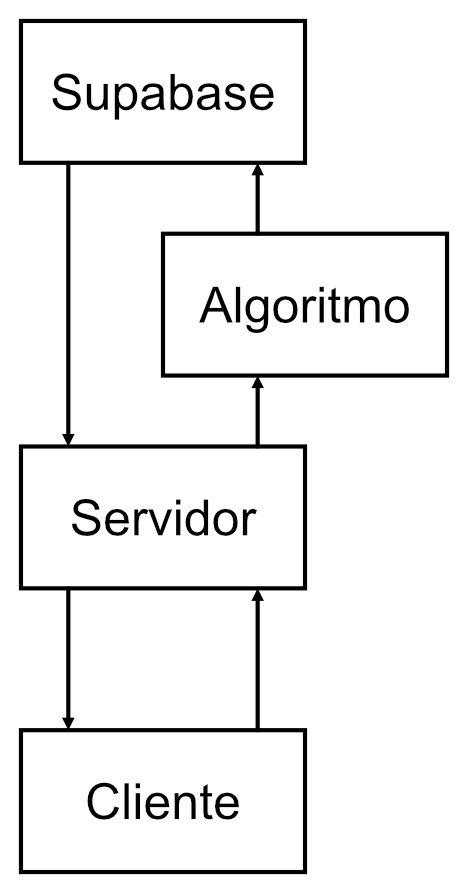
\includegraphics[width=0.2\textwidth]{Ilustraciones/desarrollo/incremento3/diseño/diagrama_flujo_por_alg_it3.jpg}
    \caption{Integración del algoritmo de cálculo de diagramas de acordes en el flujo de datos}\label{fig:diagrama_flujo_alg_it3}
\end{figure}

\textbf{Seguidamente}, se identificaron las tablas y campos necesarios para la definición de canciones, solicitudes y reportes:

\begin{itemize}
    \item \textbf{Canciones}, caracterizada por los campos:
    \begin{itemize}
        \item \textbf{Nombre}, con un máximo 64 caracteres.
        \item \textbf{Álbum}, con un máximo 64 caracteres.
        \item \textbf{Autor}, con un máximo 64 caracteres.
        \item \textbf{Género}, con hasta dos entradas, cada una con máximo 12 caracteres.
        \item \textbf{Cuerpo}, con un máximo 10.000 caracteres.
        \item \textbf{Acordes}, extraídos del \textbf{cuerpo} se representan mediante un vector generado por el algoritmo. Para cada instrumento \textit{(i.e. timple y contra)} se incluyen las variantes transpuestas del acorde desde -6 hasta +6 pasos, cada una con su nombre y vector.
        \item \textbf{Usuario}, con una clave foránea.
    \end{itemize}
    \item \textbf{Solicitudes}, similar a la tabla de canciones:
    \begin{itemize}
        \item \textbf{Nombre}, con un máximo 64 caracteres.
        \item \textbf{Álbum}, con un máximo 64 caracteres.
        \item \textbf{Autor}, con un máximo 64 caracteres.
        \item \textbf{Género}, con hasta dos entradas, cada una con máximo 12 caracteres.
        \item \textbf{Usuario solicitante}, con una clave foránea.
    \end{itemize}
    \item \textbf{Reportes}, diseñada para permitir la inclusión de objetos de reporte en el futuro:
    \begin{itemize}
        \item \textbf{Razón}, con un máximo 256 caracteres.
        \item \textbf{Estado}, con un máximo 12 caracteres.
        \item \textbf{Usuario reportado}, con unaclave foránea.
        \item \textbf{Canción reportada}, con una clave foránea.
        \item \textbf{Usuario reportador}, con una clave foránea.
    \end{itemize}
\end{itemize}

Utilizando como referencia la estructura de datos del incremento 1, se elaboró un diagrama incorporando las nuevas tablas y sus relaciones \figref{fig:diagrama_datos_i3}.

\begin{figure}[H]
    \centering
    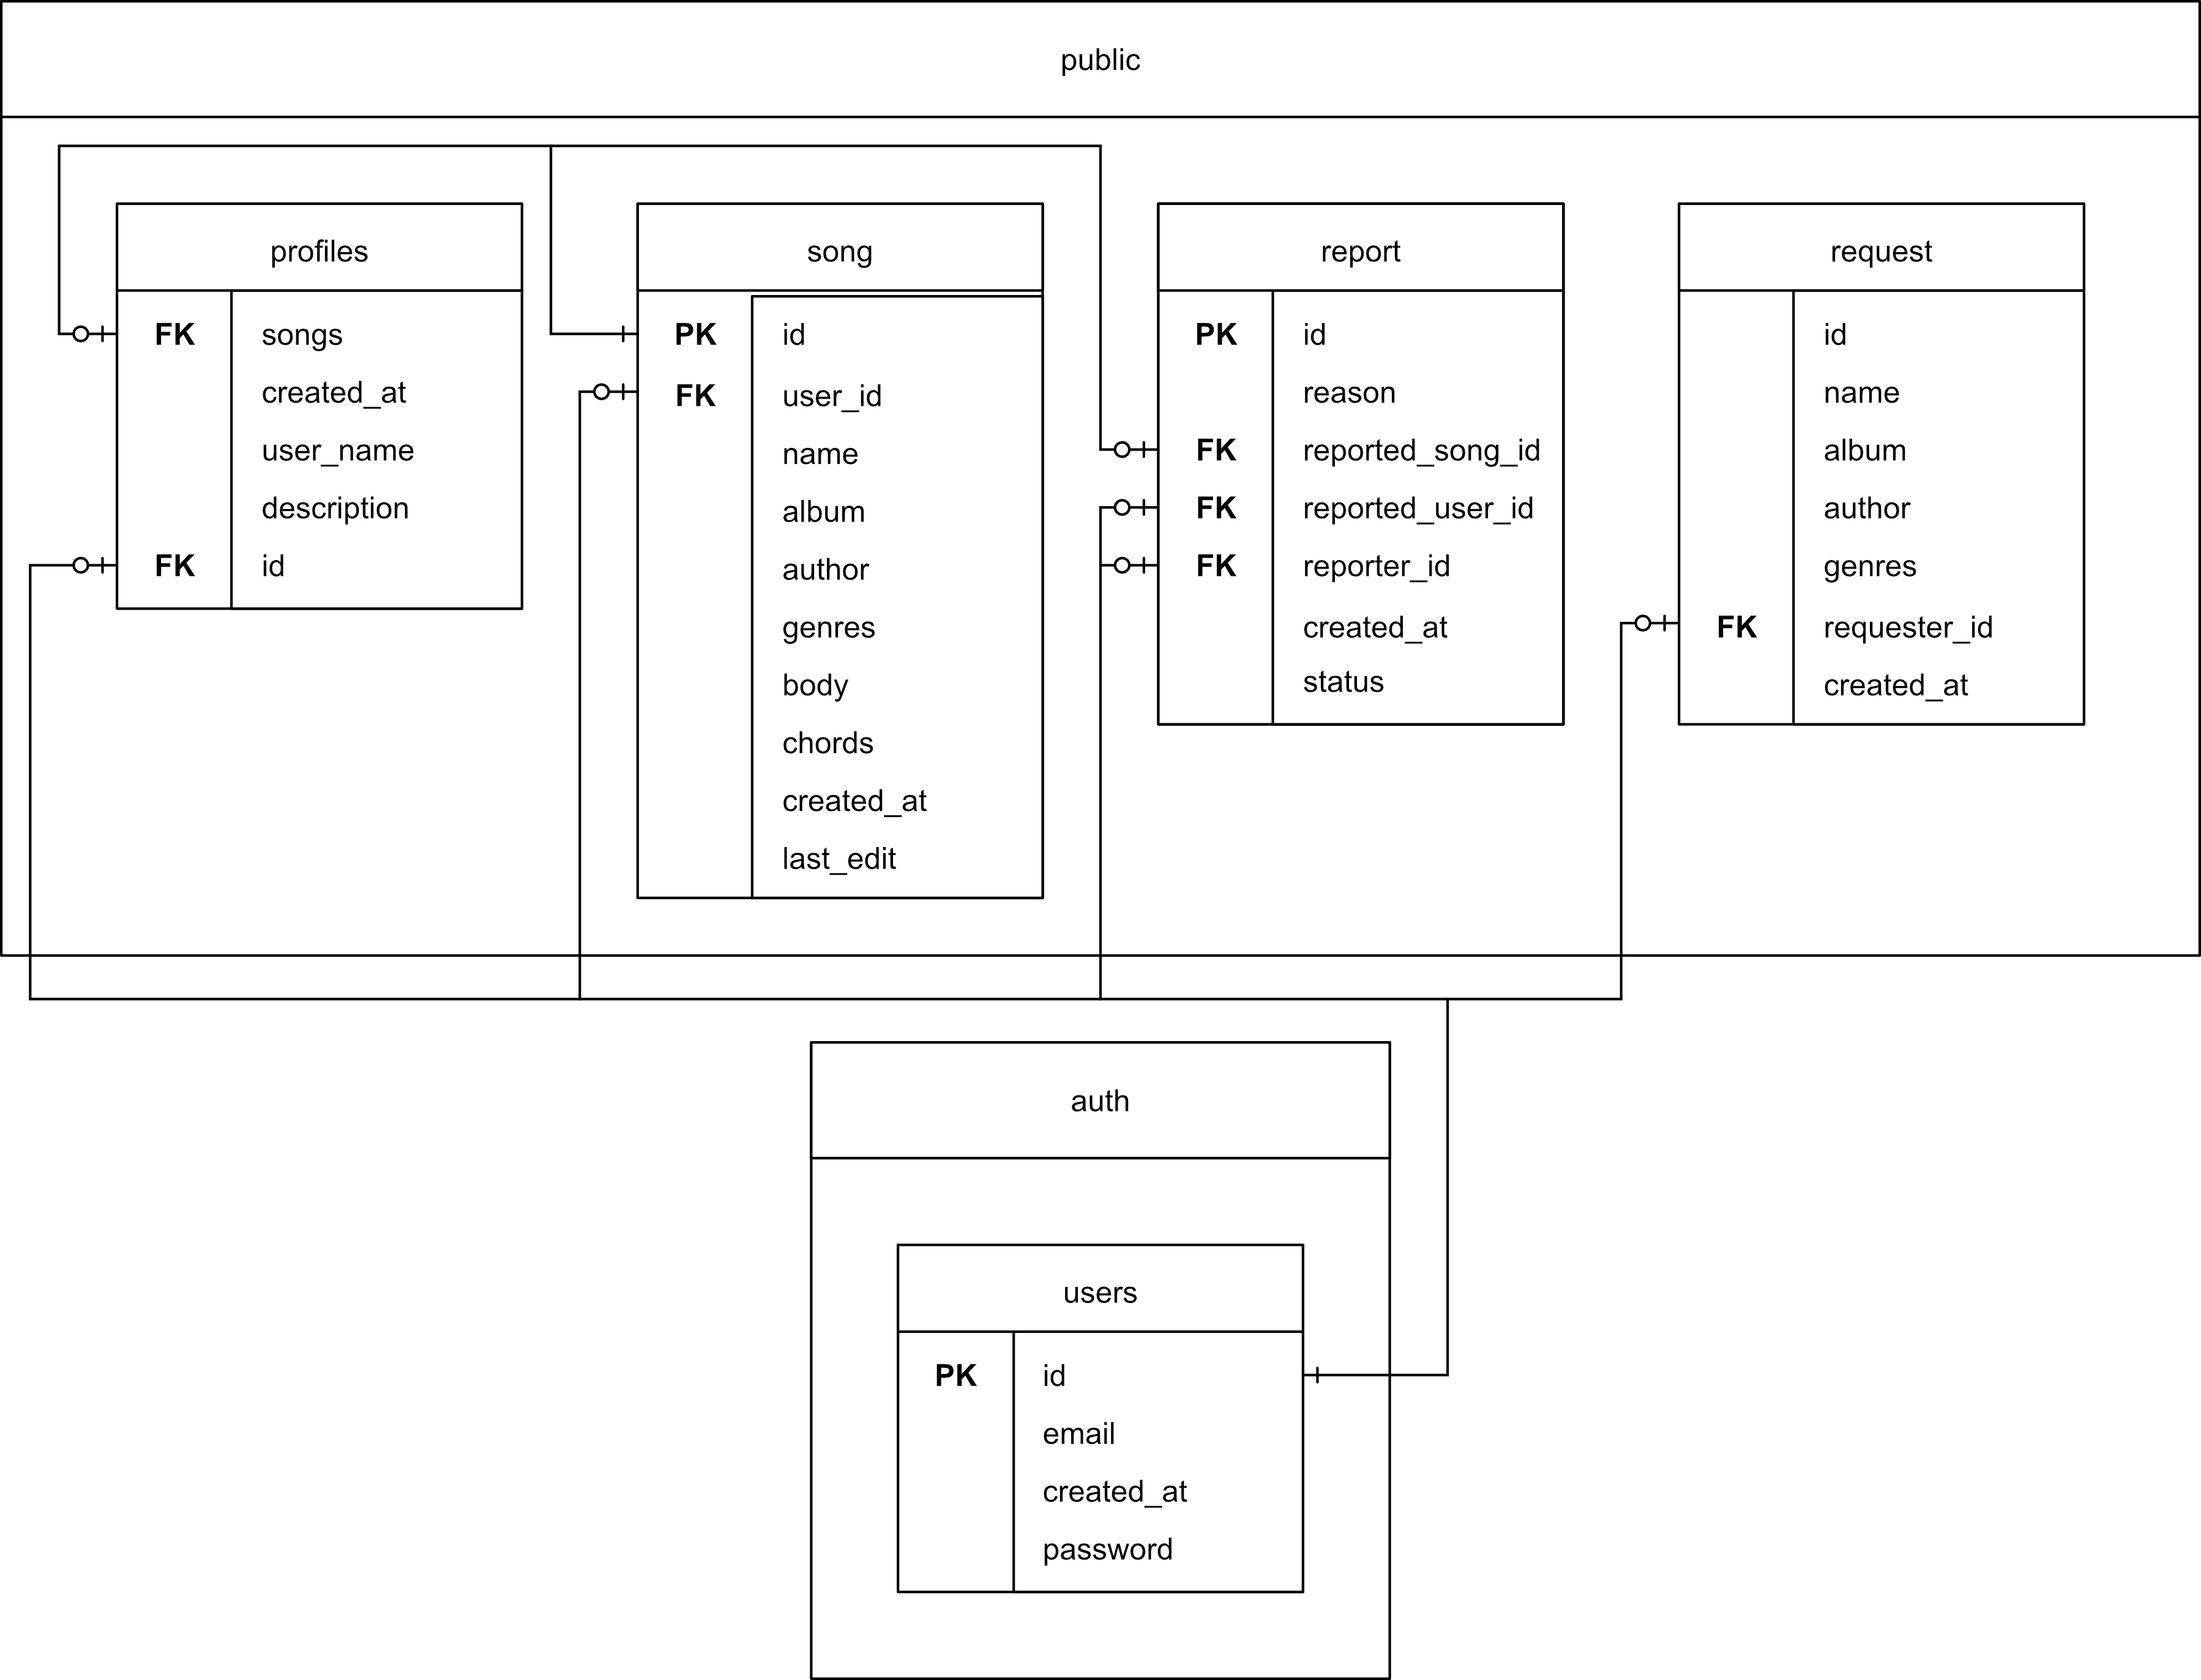
\includegraphics[width=0.8\textwidth]{Ilustraciones/desarrollo/incremento3/diseño/data_diagram_it3.jpg}
    \caption{Diagrama de estructura de datos de canciones, solicitudes y reportes}\label{fig:diagrama_datos_i3}
\end{figure}

\subsection{Diseño de interfaz}
Durante el diseño de la interfaz se diseñaron las páginas correspondinetes a: la visualización de una canción publicada, los formularios de creación y edición de canciones, la solicitud y la resolución de solicitudes, el listado de solicitudes y demás se incorporó en los perfiles del usuario una sección con la lista de publicaciones y un botón en el \textit{header} para acceder al formulacio de creación de canciones.

\textbf{En primer lugar}, con respecto a las canciones se elaboró el diseño de:

\begin{itemize}
    \item La página de una canción publicada \figref{fig:song_it3} con secciones como:
        \begin{itemize}
            \item Información general, nombre, autor, album, nombre de usuario, fecha de publicación y edición, y generos.
            \item Ajuste de la canción con utilidades para la selección de instrumento, notación musical y transposición.
            \item Lista de \gls{acorde}s presentes en la canción.
            \item Utilidad de autodesplazamiento.
            \item Letra, acordes y \gls{rasgueo}s.
        \end{itemize}
        Además, se diseñó para un acorde seleccionado, una vista flotante de su respectivo diagrama \figref{fig:song2_it3}.
    \item El formulario para la publicación de una cancion \figref{fig:new_song_it3}, con campos como: nombre de la pieza, autor, album, género, canción (letra, acordes y rasgueos) y aceptación de conformidad con las reglas de la aplicación.
    \item Un botón en el \textit{header} para acceder al formulario de creación de canciones.
    \item El formulario para la edición de una cancion \figref{fig:edit_song_it3}, con los mismos campos del formulario de creación, pero siendo unicamente modificable la canción.
\end{itemize}

\begin{figure}[H]
    \centering
    \begin{subfigure}[t]{0.20\textwidth}
        \centering
        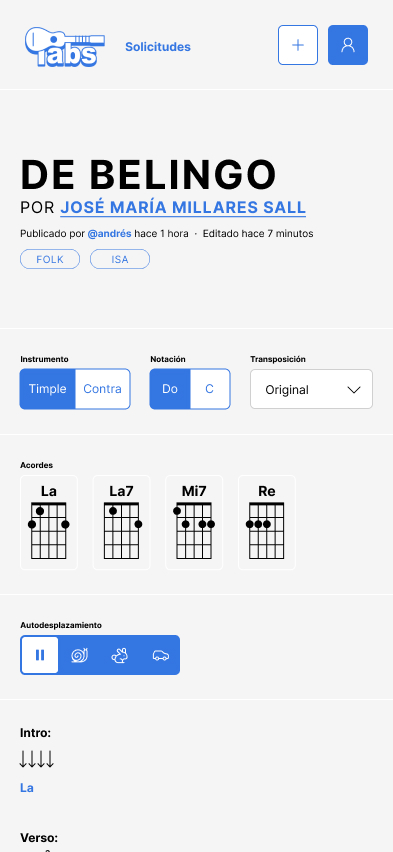
\includegraphics[width=1\textwidth]{Ilustraciones/desarrollo/incremento3/diseño/song.jpg}
        \caption{Diseño de página de canción publicada}\label{fig:song_it3}
    \end{subfigure}
    \hspace{0.5cm}
    \begin{subfigure}[t]{0.20\textwidth}
        \centering
        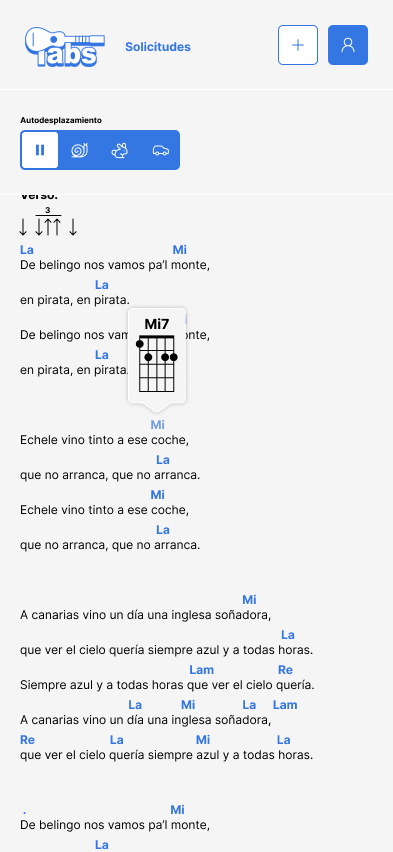
\includegraphics[width=1\textwidth]{Ilustraciones/desarrollo/incremento3/diseño/song2.jpg}
        \caption{Diseño de página de canción publicada con foco en un acorde}\label{fig:song2_it3}
    \end{subfigure}
    \hspace{0.5cm}
    \begin{subfigure}[t]{0.20\textwidth}
        \centering
        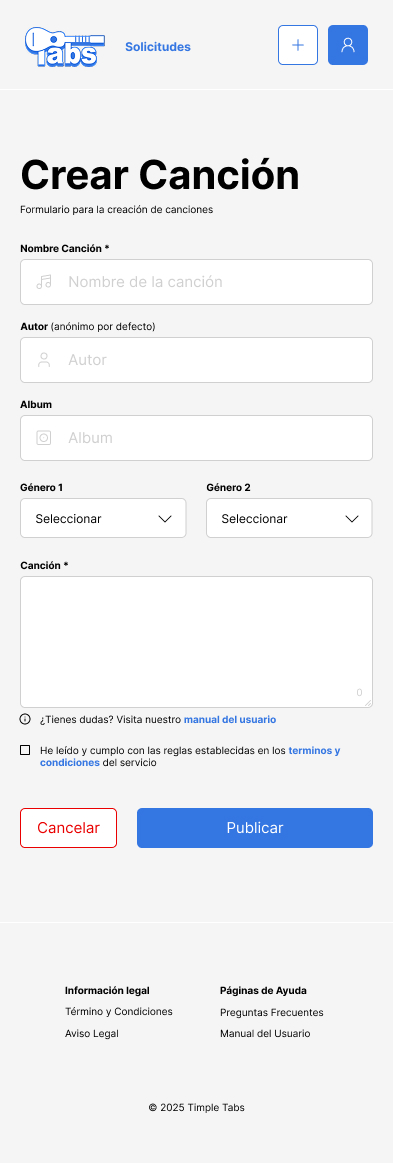
\includegraphics[width=1\textwidth]{Ilustraciones/desarrollo/incremento3/diseño/newSong.jpg}
        \caption{Diseño de página de formulario de creación de canción}\label{fig:new_song_it3}
    \end{subfigure}
    \hspace{0.5cm}
    \begin{subfigure}[t]{0.20\textwidth}
        \centering
        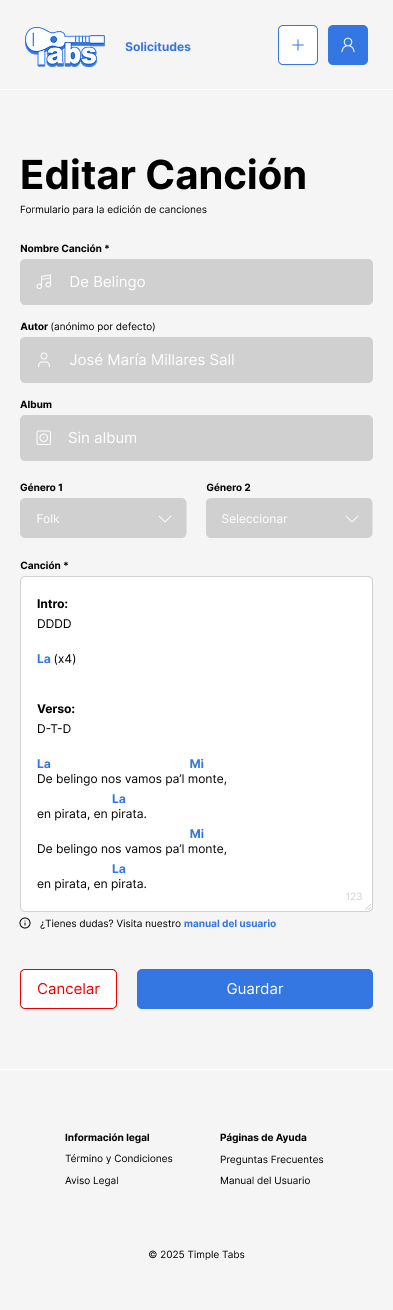
\includegraphics[width=1\textwidth]{Ilustraciones/desarrollo/incremento3/diseño/editSong.jpg}
        \caption{Diseño de página de formulario de edición de canción}\label{fig:edit_song_it3}
    \end{subfigure}
    \vspace{1em}
    \caption{Diseño de páginas relacionadas con la visualización y creación de canciones}\label{fig:song_it3}
\end{figure}

\textbf{En segundo lugar}, con respecto a la solicitud de canciones se elaboró el diseño de:

\begin{itemize}
    \item La página con el listado de solicitudes existentes \figref{fig:song_request_list_it3}, y botones para el acceso a la resolución y reporte de solicitudes. 
    \item El formulario de resolución de una solicitud seleccionada \figref{fig:song_request_form_it3}.
    \item El formulario de solicitud de una cancion \figref{fig:song_request_it3}.
\end{itemize}

\begin{figure}[H]
    \centering
    \begin{subfigure}[t]{0.20\textwidth}
        \centering
        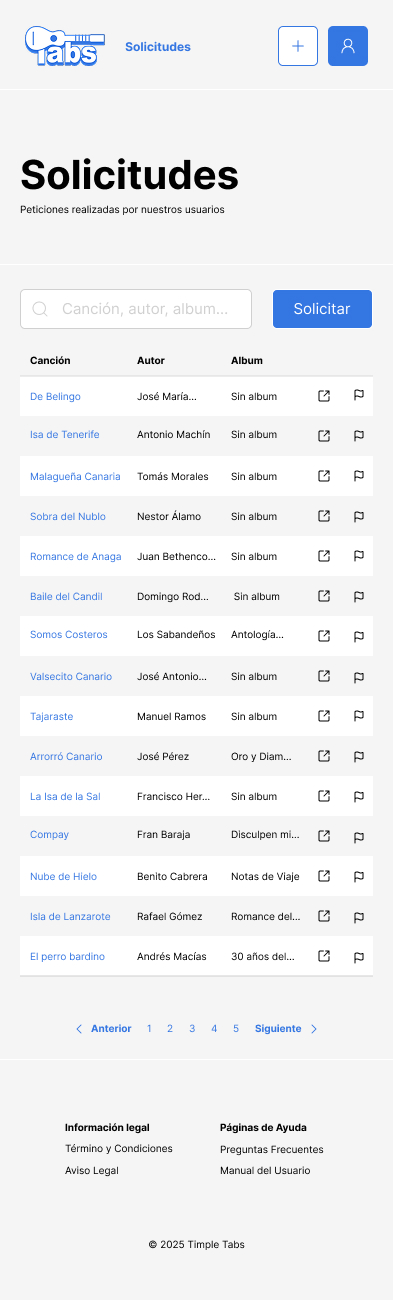
\includegraphics[width=1\textwidth]{Ilustraciones/desarrollo/incremento3/diseño/requestList.jpg}
        \caption{Diseño de página de lista de solicitudes}\label{fig:song_request_list_it3}
    \end{subfigure} 
    \hspace{0.5cm}
    \begin{subfigure}[t]{0.20\textwidth}
        \centering
        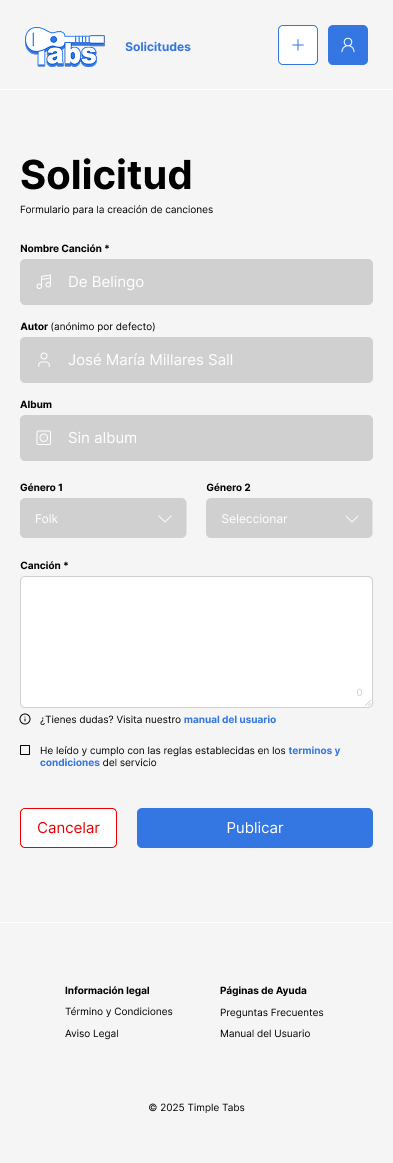
\includegraphics[width=1\textwidth]{Ilustraciones/desarrollo/incremento3/diseño/requestSubmitForm.jpg}
        \caption{Diseño de página de formulario de resolución de solicitud}\label{fig:song_request_form_it3}
    \end{subfigure}
    \hspace{0.5cm}
     \begin{subfigure}[t]{0.20\textwidth}
        \centering
        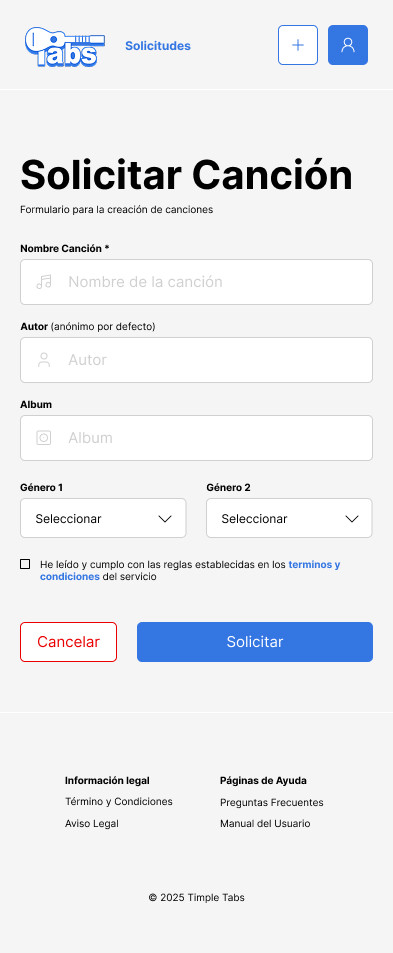
\includegraphics[width=1\textwidth]{Ilustraciones/desarrollo/incremento3/diseño/requestForm.jpg}
        \caption{Diseño de página de solicitud de cancion}\label{fig:song_request_it3}
    \end{subfigure}
    \vspace{1em}
    \caption{Diseño de páginas relacionadas con la solicitud de canciones y resolución de solicitudes}\label{fig:song_request_general_it3}
\end{figure}

\textbf{En tercer lugar}, se incorporó en los perfiles una lista de canciones publicadas por el usuario \figref{fig:song_published_it3}, y botones para el acceso a la edición, eliminación y reporte.

\begin{figure}[H]
    \centering
    \begin{subfigure}[t]{0.20\textwidth}
        \centering
        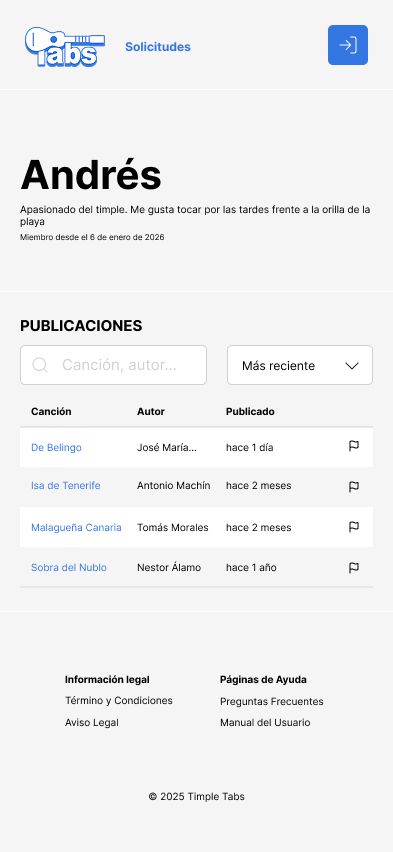
\includegraphics[width=1\textwidth]{Ilustraciones/desarrollo/incremento3/diseño/publicProfileWithSongList.jpg}
        \caption{Diseño de página principal de usuarios no registrados}\label{fig:song_published_public_it3}
    \end{subfigure}
    \hspace{0.5cm}
    \begin{subfigure}[t]{0.20\textwidth}
        \centering
        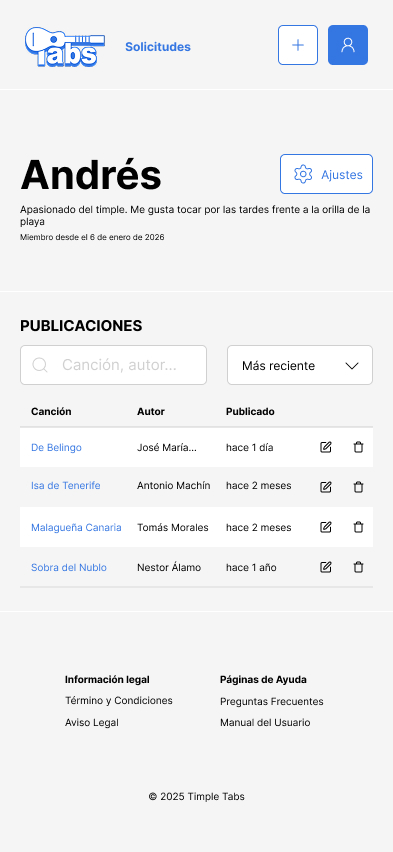
\includegraphics[width=1\textwidth]{Ilustraciones/desarrollo/incremento3/diseño/privateProfileWithSongList.jpg}
        \caption{Diseño de página de inicio de sesión}\label{fig:song_published_private_it3}
    \end{subfigure}  
    \vspace{1em}
    \caption{Diseño de página de ajustes de cuenta de usuario}\label{fig:song_published_it3}
\end{figure}

\textbf{Finalmente}, se diseñó el dialogo de reporte \figref{fig:report_it3} utilizando botones redondos de una sola opción.

\begin{figure}[H]
    \centering
    \begin{subfigure}[t]{0.20\textwidth}
        \centering
        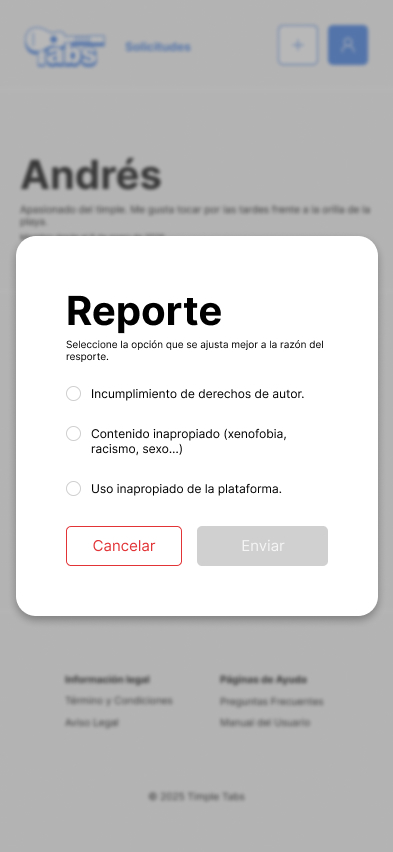
\includegraphics[width=1\textwidth]{Ilustraciones/desarrollo/incremento3/diseño/report.jpg}
        \caption{Diseño de diálogo de reporte sin selección}\label{fig:report_1_it3}
    \end{subfigure}
    \hspace{0.5cm}
    \begin{subfigure}[t]{0.20\textwidth}
        \centering
        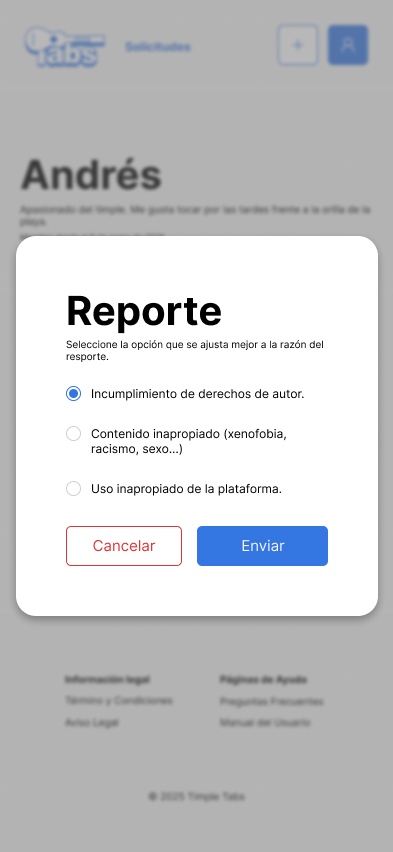
\includegraphics[width=1\textwidth]{Ilustraciones/desarrollo/incremento3/diseño/report2.jpg}
        \caption{Diseño de diálogo de reporte con una selección}\label{fig:report_2_it3}
    \end{subfigure}  
    \vspace{1em}
    \caption{Diseño de diálogo de reporte}\label{fig:report_it3}
\end{figure}